ATENCI'ON: HAY QUE RESOLVER PROBEMAS DE COMPATIBILIDAD DEL TEXTO QUE SIGUE





\section{Compacidad}

Es quizas con la noci'on de conjunto compacto donde encontraremos
las diferencias m'as grandes entre la topolog'ia de $\mathbb{R}^n$
y la de un espacio m'etrico arbitrario. En particular, ya no ser'a
v'alida la carectizaci'on de compacto como cerrado y acotado. Para
obtener una caracterizaci'on necesitaremos un concepto m'as fuerte
que la acotaci'on, este ser'a el de conjunto \textbf{totalmente
acotado} y, a la vez, un concepto m'as fuerte que el de conjunto
cerrado y en este caso usaremos la de conjunto completo.

Es interesante hacer notar que, en topolog'ia, interesan aquellas
propiedades que se preservan por homeomorfismos. En este sentido
vemos que la noci'on de conjunto cerrado acotado no se preserva
por este tipo de aplicaciones (claro est'a, los espacios m'etricos
involucrados deber'ian ser distintos que $\mathbb{R}^n$ con la
m'etrica euclidea). Por ejemplo, como ya hemos visto, la identidad
es un homeomorfismo de $(\mathbb{R}^n,d)$, con $d$ la m'etrica
euclidea, en $(\mathbb{R}^n,d_1)$, con
\[
	d_1(x,y)=\frac{d(x,y)}{1+d(x,y)}.
\]
Ahora bien, como $0\leq d_1<1$ cualquier conjunto de
$\mathbb{R}^n$ tiene di'ametro, respecto a $d_1$ menor o igual a
$1$ y, por ende, cualquier conjunto es acotado. Sin embargo, no
todo conjunto es acotado respecto a la m'etrica euclidea. Por otra
parte $\mathbb{R}^n$ es cerrado en ambas m'etricas, pues es el
conjunto total. Vemos as'i que el concepto de conjunto cerrado y
acotado no necesariamente se preserva por homeomorfismos lo que
relativiza su importancia.



\begin{definicion}  Diremos que un conjunto $A$ de un e.m. $(X,d)$
es totalmente acotado
si para cada $\epsilon>0$ existe una cantidad finita de conjuntos
de di\'ametro menor que $\epsilon$ cuya uni\'on contiene a  $A$.
En otras palabras existen conjuntos $A_i$, $i=1,...,n$, con
$\delta(A_i)<\epsilon$ que satisfacen:
\[
	A\subset \bigcup\limits_{i=1}^nA_i.
\]
\end{definicion}


\begin{ejercicio}\label{ejer,subpreespre} Demostrar que un
subconjunto de un conjunto totalmente acotado es totalmente
acotado.
\end{ejercicio}


Veamos algunos ejemplos de conjuntos totalmente acotados y de
conjuntos que no lo son.

\begin{ejemplo} Cualquier intervalo acotado de $\rr$ es
totalmente acotado. Para justificar esta aseveraci\'on, tomemos
$\epsilon>0$ y un intervalo cualquiera de extremos $a$ y $b$.
Elijamos $n$ suficientemente grande para que $1/n<\epsilon$.
Entonces los conjuntos
\[
	I_k:=\Big[\frac{k}{n},\frac{k+1}{n}\Big]\quad ,k=0,\ldots,n-1,
\]
satisfacen la definici\'on.
\end{ejemplo}

\begin{ejemplo}\label{ejem,cubpre} Cualquier conjunto  acotado en el
espacio euclideo $\rr^n$ es totalmente acotado. Sea
$A\subset\rr^n$ un conjunto acotado, entonces $A$  est\'a
contenido en un cubo de la forma $C:=[-m,m]\times\dots\times
[-m,m]=[-m,m]^n$. En virtud del Ejercicio \vref{ejer,subpreespre}
es suficiente demostrar que $C$ es totalmente acotado. Sea
$\epsilon>0$. Tomemos $k$ suficientemente grande para que
\begin{equation}\label{eq,defk}
	\frac{2\sqrt{n}m}{\epsilon}<k
\end{equation}
Ahora, partimos cada intervalo $[-m,m]$ en $k$ subintervalos de la
misma longitud $1/k$.

\begin{figure}[h]
\begin{center}
	\psfrag{a}{$\frac{2m}{k}$}
	\psfrag{b}{$\frac{2\sqrt{2}m}{k}$}
	\includegraphics[height=6cm, width=10cm]{cubpre.eps}
	\caption{Construcci\'on del Ejemplo
	\ref{ejem,cubpre}}\label{fig,cubpre}
\end{center}
\end{figure}

Como puede observarse en la Figura \ref{fig,cubpre}, nos quedan
determinados $k^n$ cubos que cubren el cubo $C$. Cada uno de estos
cubos m\'as chicos tiene di\'ametro $2\sqrt{n}m/k$, por
consiguiente, por la desigualdad \ref{eq,defk}, el di\'ametro de
ellos es menor que $\epsilon$.
\end{ejemplo}

No es cierto, en general, que todo conjunto acotado en un e.m. sea
totalmente acotado. Los siguientes ejemplos muestran esto.

\begin{ejemplo} Sea $(X,d)$ un e.m. discreto con $X$ infinito. El
conjunto $X$ es acotado, de hecho $\delta(X)=1$; sin embargo no
podemos cubrir $X$ con conjuntos de di\'ametro menor que 1/2
(cualquier n\'umero menor que 1 servir\'{\i}a). Esto ocurre debido
a que si un conjunto en un e.m. discreto tiene m\'as de un
elemento entonces su di\'ametro es 1. As\'{\i}, si cubrimos $X$
con una cantidad finita de conjuntos, alguno de los conjuntos del
cubrimiento necesariamente tiene m\'as de un elemento, de lo
contrario $X$ ser\'{\i}a finito, por consiguiente el di\'ametro de
este conjunto es 1 y no puede ser menor que $1/2$.
\end{ejemplo}

\begin{ejemplo}\label{ejem,contnopre} En $C([0,1])$, con la m\'etrica
 del Ejemplo
\vref{ejem,distsobrecont}, la bola cerrada $K(0,1)$ (0 denota la
funci\'on que es constantemente igual a 0) no es un conjunto
totalmente acotado. Para ver esto definimos la siguiente
funci\'on:

\[
	f(x):=\left\{%
\begin{array}{ll}
	4(x-\frac12), & \hbox{si $\frac12\leq x\leq \frac34$;} \\
	-4(x-1), & \hbox{si $\frac34\leq x\leq 1$;} \\
	0, & \hbox{para los restantes $x$;} \\
\end{array}
\right.
\]
y la siguiente sucesi\'on de funciones $f_n(x):=f(2^nx)$. En la
Figura \ref{fig,contnopre} puede verse las gr\'aficas de algunas
de las funciones de la sucesi\'on.

\begin{figure}[h]
\begin{center}
	\psfrag{f1}{$f_1$}
	\psfrag{f2}{$f_2$}
	\psfrag{f3}{$f_3$}
	\psfrag{f4}{$f_4$}
	\psfrag{1}{$1$}
	\psfrag{12}{$\frac12$}
	\psfrag{14}{$\frac14$}
	\psfrag{18}{$\frac18$}
	\psfrag{116}{$\frac{1}{16}$}
	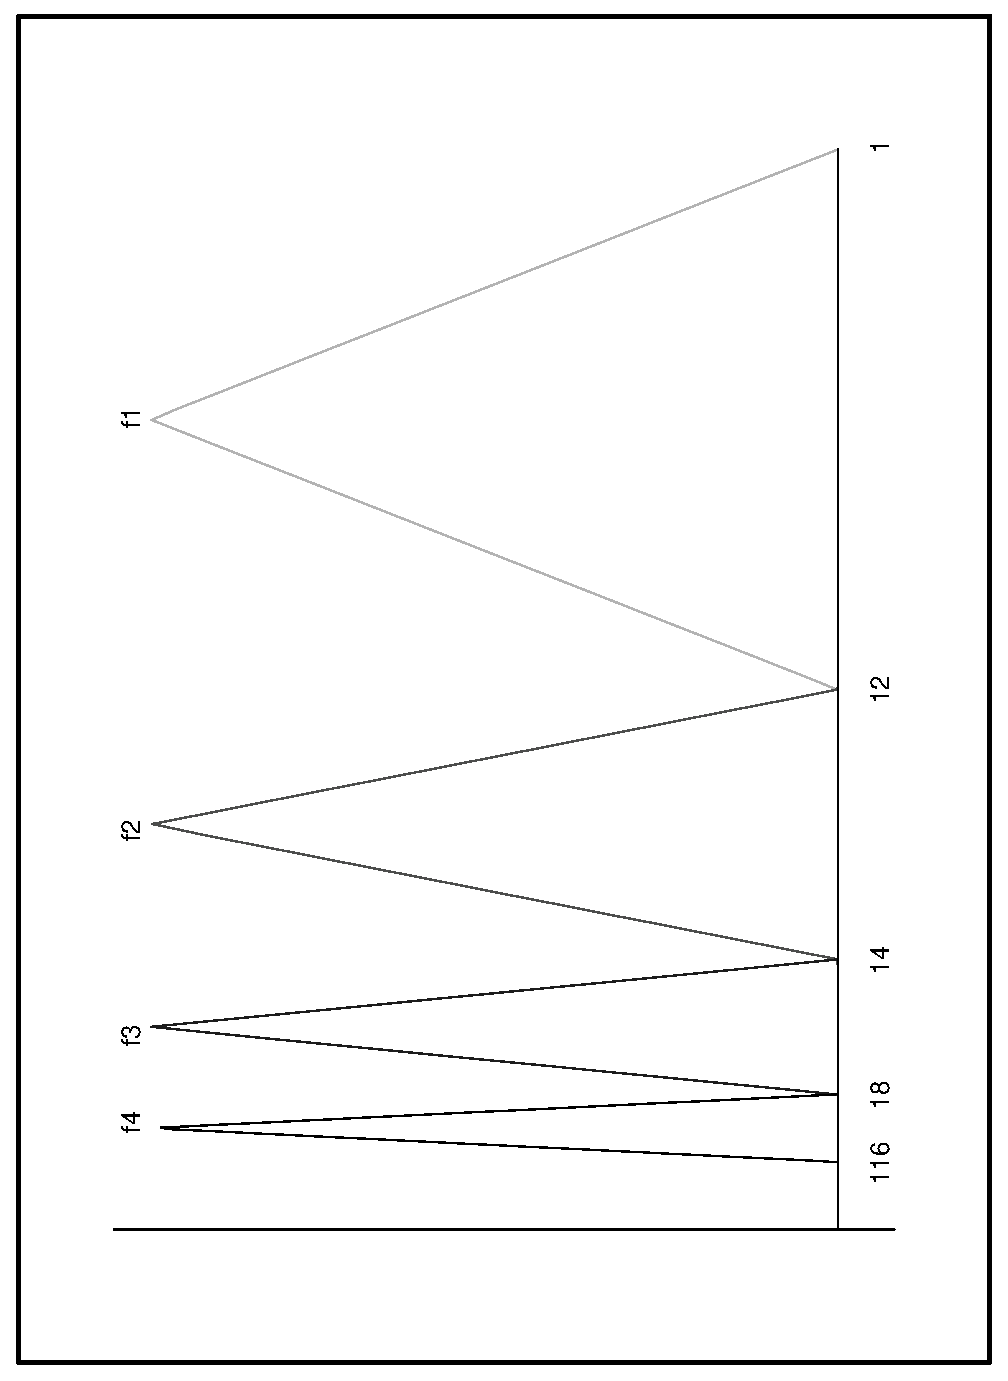
\includegraphics[height=12cm,
	width=7cm,angle=-90]{noprecom.eps}
	\caption{Funciones del Ejemplo
	\ref{ejem,contnopre}}\label{fig,contnopre}
\end{center}
\end{figure}

Puede demostrarse que la distancia de cualquiera de las funciones
de la sucesi\'on a otra es igual a 1 y que $f_n\in K(0,1)$. Sea
$C:=\{f_n:n\in\nn\}$, observemos que como subespacio $C$ resulta
ser un e.m. discreto, as\'{\i}, por el Ejemplo anterior y el
Ejercicio \vref{ejer,subpreespre}, $\C{B(0,1)}$ no puede ser
totalmente acotado.
\end{ejemplo}

\begin{ejemplo} Hay una interesante conexi'on de la total
acotaci'on con la dimensi'on. Para introducirla, veamos
 cuantas bolas abiertas de radio
$1/2$, en $\mathbb{R}^n$ con la m'etrica euclidea,
se necesitan, al menos,  para cubrir la bola cerrada $K(0,1)$.
Denotemos por $e_j$ los vectores can'onicos
\[
	e_j:=(0,\ldots,1,\ldots,0),
\]
donde el $1$ est'a en el lugar $j$. Notes'e que $e_j\in K(0,1)$ y que:
\[
	d(e_j,e_i)=\sqrt{2}\quad i\neq j.
\]
De modo que, si $i\neq j$ entonces $e_i$ y $e_j$ no pueden estar
en una misma bola de radio $1/2$. De lo contrario, si $e_i,e_j\in
B(x,1/2)$, entonces
\[
	d(e_i,e_j)\leq d(e_i,x)+d(x,e_j)<1<\sqrt{2},
\]
que es una contradicci'on. De esta manera si cubrimos la bola cerrada
$K(0,1)$ por bolas abiertas de radio $1/2$ necesitaremos, al menos,
$n$ de estas bolas. Es decir, la cantidad de estas bolas crece cuando aumenta
la dimensi'on $n$. Esta observaci'on nos lleva a conjeturar que si
buscamos un espacio vectorial de dimensi'on infinita\footnote{Esto significa
que no tiene una base finita} tenemos chances de construir conjuntos acotados,
en particular la bola $K(0,1)$, que no son totalmente acotados.

\begin{ejercicio} Demostrar que en $l_2$ la bola cerrada $K(0,1)$
no es totalmente acotada.
\end{ejercicio}
\end{ejemplo}


Recordemos que, en un e.m. $(X,d)$, una familia de conjuntos
abiertos $\{U_i\}_{i\in I}$ es un cubrimiento por abiertos de
$A\subset X$ si
\[
	A\subset\bigcup\limits_{i\in I}U_i.
\]
\begin{definicion} Un subconjunto $A$ de un e.m. $(X,d)$ se dir\'a
\textbf{compacto} si, y solo si, todo cubrimiento por abiertos de
$A$ tiene un subcubrimiento finito. Es decir, si $\{U_i\}_{i\in
I}$ es un cubrimiento  de $A$, existe un conjunto finito $F\subset
I$ tal que $\{U_i\}_{i\in F}$ es un cubrimiento de $A$.
\end{definicion}



\begin{ejercicio} Demostrar que un espacio m'etrico discreto es compacto
si, y solo si, es finito.
\end{ejercicio}

\begin{ejercicio} Demostrar que un conjunto totalmente acotado es
acotado.
\end{ejercicio}



\begin{ejercicio}\label{ejer,precantfinibolas} Demostrar que $X$ es totalmente acotado si, y
solo si, para cada $\epsilon>0$ podemos cubrir $X$ por una cantidad
finita de bolas de radio $\epsilon$.
\end{ejercicio}

\begin{ejercicio} Demostrar que un conjunto compacto es cerrado y
acotado.
\end{ejercicio}

\begin{ejercicio} Demostrar que si $f:(X,d)\to (Y,d')$ es continua
y $X$ compacto entonces $f(X)$ es compacto. Como corolario,
demostrar que si $f:X\to\mathbb{R}$ y $X$ es compacto entonces $f$
alcanza un m'aximo y un m'inimo.
\end{ejercicio}

\begin{teorema}[Caracterizaci'on de compacidad en espacios m'etricos]
 Sea $(X,d)$ un  espacio m'etrico. Entonces son
equivalentes:

\begin{enumerate}
\item\label{inc,compacto} $X$ es compacto;
\item\label{inc,toacotadoycomp} $X$ es totalmente acotado y
completo.
\item\label{inc,subs} Toda sucesi'on en $X$ tiene una subsucesi'on
convergente.
\end{enumerate}
\end{teorema}
\begin{demo} Veamos que
\ref{inc,compacto}$\Rightarrow$\ref{inc,subs}. Por el absurdo
supongamos que existe una sucesi'on $\{a_n\}$ en $X$ que no tiene
ninguna subsucesi'on convergente. Definamos $\Gamma$ como la
colecci'on de todos los conjuntos abiertos $G$ de $X$ tales que
$G$ tiene una cantidad finita de elementos de la sucesi'on, es
decir:
\[
G\in\Gamma\Leftrightarrow \#\{n:a_n\in G\}<\infty.
\]
Vamos a probar que $\Gamma$ es un cubrimiento de $X$. Supongamos
que $x\in X$ y $x\notin G$ para todo $G\in\Gamma$. De modo que,
por definici'on, cada abierto que contiene a $x$ contiene
infinitos t'erminos de la sucesi'on $\{a_n\}$. En particular,
podemos encontrar $n_1$ tal que $a_{n_1}\in B(x,1)$. Ahora podemos
encontrar $n_2>n_1$ tal que $a_{n_2}\in B(x,\frac12)$. Y as'i
continuamos, constru'imos una subsucesi'on $a_{n_k}$ tal que
$a_{n_k}\in B(x,\frac1k)$. Lo que implica que $a_{n_k}$ converge a
$x$, contradiciendo nuestra suposici'on. De esta manera,
$\Gamma$ es un cubrimiento de $X$. Sea $G_i$, $i=1,\ldots,n$, un
subcubrimiento finito de $X$. Es decir
\[
	X=G_1\cup\dots\cup G_n.
\]
Como cada $G_i$, $i=1,\ldots,n$, tiene una cantidad finita de
t'erminos de la sucesi'on, conclu'imos que $X$
contiene una cantidad finita de t'erminos de la sucesi'on, lo que,
claro est'a, no puede ocurrir. Esto finaliza la demostraci'on de
\ref{inc,compacto}$\Rightarrow$\ref{inc,subs}.

Demostremos ahora que \ref{inc,subs}$\Rightarrow$
\ref{inc,toacotadoycomp} empezando por ver que $X$ es totalmente
acotado. Nuevamente procedemos por el absurdo, suponiendo que $X$
no es totalmente acotado. Esto implica que existe un $\epsilon>0$
tal que $X$ no se puede cubrir con una cantidad finita de
conjuntos de di'ametro $\epsilon$. Sea $a_1$ cualquier punto de
$X$. Como $B(a_1,\epsilon)$ no cubre $X$, existe $a_2\in
X-B(a_1,\epsilon)$. Como $B(a_i,\epsilon)$, $i=1,2$, no cubren
$X$, existe un $a_3\in X-\bigl(B(a_1,\epsilon)\cup
B(a_2,\epsilon)\bigr)$. Continuando de esta forma, contru'imos una
sucesi'on $a_n$ tal que
\[
	a_n\in X-\big(B(a_1,\epsilon)\cup\dots\cup
	B(a_{n-1},\epsilon)\big).
\]
De esta forma tendremos que:
\[
	d(a_i,a_j)\geq \epsilon\quad\hbox{para $i\neq j$}.
\]
Por hip'otesis la sucesi'on $a_n$ tiene una subsucesi'on convergente,
en particular esta subsucesi'on ser'a  de Cauchy. No obstante la desigualdad
anterior implica que ninguna subsucesi'on de $\{a_n\}$ puede
ser de Cauchy, contradicci'on que prueba que $X$ es totalmente acotado.

Veamos ahora que $X$ es completo. Sea $\{a_n\}$ una sucesi'on de
Cauchy en $X$. Podemos extraer una subsucesi'on $\{a_{n_k}\}$
convergente a un $a\in X$. Sea $\epsilon>0$. Puesto que $\{a_n\}$
es de Cauchy, pondemos encontrar $N>0$ tal que si $n,m>N$ entonces:
\begin{equation}\label{eq,conddecauchy}
	d(a_n,a_m)<\frac{\epsilon}{2}.
\end{equation}
Como $a_{n_k}$ converge a $a$, podemos encontrar un $n_k$ lo
suficientemente
grande para que $n_k>N$ y:
\[
	d(a_{n_k},a)<\frac{\epsilon}{2}.
\]
As'i, usando \eqref{eq,conddecauchy},  tenemos que para $n>N$:
\[
	d(a_n,a)\leq d(a_n,a_{n_k})+d(a_{n_k},a)<\epsilon.
\]
Por 'ultimo veamos que \ref{inc,toacotadoycomp}
$\Rightarrow$\ref{inc,compacto}. Para este fin elijamos un
cubrimiento $\{G_{\lambda}\}_{\lambda\in L}$ arbitrario de $X$.
Supongamos que este cubrimiento no tiene un subcubrimiento finito.
Como $X$ es totalmente acotado, acorde al Ejercicio
\ref{ejer,precantfinibolas}, podemos cubrir a $X$ por una cantidad
finita de bolas de radio $1$. Alguna de estas bolas no se podr'a
cubrir por una cantidad finita de $G_{\lambda}$, de lo contrario,
si todas se cubren por una cantidad finita, como hay una cantidad
finita de estas bolas, podr'iamos cubrir $X$ por una cantidad
finita de $G_{\lambda}$. Llamemos $B(x_1,1)$ a la bola que no se
cubre por finitos $G_{\lambda}$. Como $B(x_1,1)$ es totalmente
acotado, podemos aplicar la construcci'on anterior a $B(x_1,1)$ en
lugar de $X$ y con bolas de radio $1/2$, en lugar de $1$,
obteniendo de esta forma una bola $B(x_2,1/2)$ que no se cubre por
una cantidad finita de $G_{\lambda}$. Adem'as podemos suponer que
$B(x_2,1/2)\cap B(x_1,1)\neq \emptyset$, de lo contrario no
hubiera tenido sentido usar la bola $B(x_2,1/2)$ para cubrir
$B(x_1,1)$. Continuamos de esta forma y producimos una sucesi'on
$B(x_n,1/2^n)$ (aqu'i no basta que los radios tiendan a cero, sino
que es necesario que la serie de radios converja) de bolas tales
que ninguna de ellas se puede cubrir por una cantidad finita de
$G_{\lambda}$. Veamos que la sucesi'on $x_n$ es de Cauchy.   Para
esto tomemos
\[
	z_n\in B\Big(x_n,\frac{1}{2^n}\Big)\cap B\Big(x_{n+1}
	,\frac{1}{2^{n+1}}\Big).
\]
Entonces
\[
	d(x_n,x_{n+1})\leq d(x_n,z_n)+d(z_n,x_{n+1})<
	\frac{1}{2^n}+\frac{1}{2^{n+1}}<\frac{1}{2^{n-1}}.
\]
Lo que permite utilizar el criterio de comparaci'on para
la convergencia de series para demostrar que:
\[
	\sum\limits_{n=1}^{\infty}d(x_n,x_{n+1})<\infty.
\]
Acorde a un ejercicio de la pr'actica, esto implica que $\{x_n\}$ es
de Cauchy, por ende converge a alg'un $x_0\in X$. Como $G_{\lambda}$
es un cubrimiento, existe $\lambda_0$ tal que $x_0\in G_{\lambda_0}$. Como
$G_{\lambda_0}$ es abierto, existe un $r>0$ tal que
\begin{equation}\label{eq,dalecasillegamos}
	B(x_0,r)\subset G_{\lambda_0}.
\end{equation}
Puesto que $x_n$ converge a $x_0$ y $1/2^{n-1}$ converge a 0,
podemos hallar $n$ lo suficientemente grande para que:
\begin{equation}\label{ufamecanse}
	d(x_n,x_0)<\frac{r}{2}\quad\hbox{y}\quad
	\frac{1}{2^{n-1}}<\frac{r}{2}.
\end{equation}
Veamos que esto, \eqref{ufamecanse} y \eqref{eq,dalecasillegamos}
implica que:
\begin{equation}\label{casicasi}
	B\Big(x_n,\frac{1}{2^n}\Big)\subset B(x_0,r)\subset G_{\lambda_0}.
\end{equation}
En efecto, si:
\[
	 y\in B\Big(x_n,\frac{1}{2^n}\Big),
\]
entonces
\[
	d(y,x_0)\leq d(y,x_n)+d(x_n,x_0)<\frac{1}{2^n}+\frac{r}{2}<r,
\]
lo que prueba \eqref{casicasi}, siendo, adem'as, esta inclusi'on
una contradicci'on puesto que estamos cubriendo la bola
$B(x_n,1/2^n)$ por un s'olo $G_{\lambda}$, recordemos que estas
bolas no se cubr'ian por finitos $G_{\lambda}$. (ya terminamos,
!`por fin!)
 \end{demo}

 \begin{ejercicio} Utilizar la siguiente ``idea'' para dar una
 demostraci'on alternativa de que compacto implica completo. Tomar
 una suseci'on de Cauchy $\{a_n\}$ en $X$. De la desigualdad

 \[
	|d(x,a_n)-d(x,a_m)|\leq d(a_n,a_m)\quad n,m\in\mathbb{N}\,\,
	x\in X
 \]
 conclu'ir que $d(x,a_n)$ es una sucesi'on de Cauchy en
 $\mathbb{R}$ y de esto que la siguiente funci'on esta bien
 definida:
\[
	f(x):=\lim\limits_{n\to\infty}d(x,a_n).
\]
Notar que $f:X\to\mathbb{R}$ y por ende $f$ alcanza un m'inimo en
alg'un $a\in X$. Por 'ultimo demostrar que $a$ es el l'imite de
$a_n$.
\end{ejercicio}

\section{Conexi'on}La definici'on de conjunto \textbf{conexo},
\textbf{arco conexo} es id'entica a la que ya hemos estudiado. Los
conjuntos conexos, as'i definidos, satisfacen las mismas
propiedades que ya observamos para la m'etrica euclidea, con una
excepci'on. El hecho que valga las mismas propiedades nos permite
definir el concepto de \textbf{componente conexa} de la misma
forma que lo hicimos para $\mathbb{R}^n$.

La propiedad que no continua valiendo, en espacios m'etricos en
general, es aquella que afirmaba que las componentes conexas de
conjuntos abiertos eran abiertas. Esto es as'i pues en la
demostraci'on de tal propiedad utilizamos que una bola era un
conjunto conexo y por el siguiente ejercicio:

\begin{ejercicio} Encontrar un ejemplo de espacio m'etrico que
tenga bolas disconexas.
\end{ejercicio}

Para conservar tal propiedad podr'iamos ``pedir'' la hip'otesis que
las bolas sean conexas. No obstante observaremos que en tal demostraci'on
podr'iamos haber utilizado cualquier entorno conexo que fuera bola o no.
Esto nos lleva a la siguiente definici'on:

\begin{definicion} Un espacio m'etrico $(X,d)$ se llama
\textbf{localmente conexo} si para todo $x\in X$ y $r>0$
existe un entorno conexo $V$ de $x$ tal que $V\subset B(x,r)\subset X$.
\end{definicion}

$\mathbb{R}^n$ es localmente conexo, podemos utilizar como $V$ la
 misma bola que aparece en la definici'on anterior. Lo curioso del
 caso es que hay espacios m'etricos $(X,d)$ tales que $X$ es conexo
 y, sin embargo, $X$ no es localmente conexo.

 \begin{ejemplo} Sea $X=\mathbb{Q}\times\mathbb{R}\cup \{(x,0):x\in\mathbb{R}\}$
 y consideremos este $X$ como subespacio de $\mathbb{R}^2$. En la
 figura \ref{noloccon} hemos hecho un bosquejo, est'a claro que es
 imposible lograr exactitud, del gr'afico $X$.
 \begin{center}
\begin{figure}[h]
 \psset{unit=1mm}
  \begin{pspicture}(0,0)(100,60)
 \psset{linewidth=1}
  \multirput{0}(0,0)(2,0){26}{\psline(0,0)(0,50)}
 \rput(0,0){\psline(0,25)(50,25)}
  \psset{linewidth=.5}
 \pscircle(25,40){8}

\rput(40,-40){
 \scalebox{2}{
\psclip{\pscircle(25,40){8}
 }

  \multirput{0}(0,0)(2,0){26}{\psline(0,0)(0,50)}
 \rput(0,0){\psline(0,25)(50,25)}
  \psset{linewidth=.5}
 \pscircle(25,40){8}
\endpsclip  }
}
\psline[linestyle=dashed](24,32)(90,24)
\psline[linestyle=dashed](24,47.5)(88,55)
\rput(116,54){$B(x,r)\cap X$}
 \end{pspicture}
 \caption{El subespacio $X$}\label{noloccon}
 \end{figure}
 \end{center}

Notes'e que si tomamos un punto en $X$ pero no sobre el eje horizontal
y consideramos una bola de centro $x$ y un radio suficientemete chico
de modo que la bola no interseque el mencionado eje, entonces
$B(x,r)\cap X$ est'a compuesto de un conjunto de segmentos verticales
disconexos entre si.  Si ahora buscamos un conjunto conexo $V$ tal que
$V\subset B(x,r)$ notaremos que $V$ deber'ia ser un subconjunto de alguno de los
segmentos verticales, precisamente de aquel segmento que tenga el $x$ dentro
de si, pero tal $V$ no ser'a un entorno. Lo que prueba que el espacio $(X.d)$
no es localmente conexo.

\end{ejemplo}

\begin{ejercicio} Demostrar que el espacio m'etrico $(X,d)$ es
localmente conexo si, y s'olo si, las componentes conexas de conjuntos
abiertos son abiertas.
\end{ejercicio}

\begin{ejercicio} Sea $(X,d)$ un espacio m'etrico localmente
conexo y compacto. Demostrar que $X$ tiene, a lo sumo, una
cantidad finita de componentes.
\end{ejercicio}

\begin{ejercicio} Sea ${X,d}$ un espacio m'etrico homeomorfo a
$\mathbb{Z}$ demostrar que las componentes conexas de $X$ son
conjuntos unitarios. Este tipo de espacios se llaman totalmente
disconexos. \end{ejercicio}
